\section{Testbox und Material}
Wie in Abschnitt~\ref{sec:testbox} angef\"uhrt, kann das Modell f\"ur die Simulationen in Grundz\"ugen aus der Bachelorarbeit von Denys Bast~\cite{bast2017ba} \"ubernommen werden. Die Modellierung der Testbox mitsamt Ringkern wurde dabei in mehreren Schritten durchgef\"uhrt. Die W\"ande der Testbox wurden mit idealem Kupfer modelliert. Ebenso wurde die Einkopplung und der Innenleiter durch die Box mit idealem Kupfer dargestellt und die Dimensionen der Verbindung entsprechend angepasst. Die Holzkonstruktion zur Halterung der Rinkerne ist im Urspr\"unglichen Modell nicht modelliert, der Ringkern h\"angt dort also in der Luft.
\par

F\"ur die Simulation sind auch die genauen dissipativen Daten des Ringkern Material wichtig. Um diese zu ermitteln werden als erstes die Ringkernimpedanz $Z_{rk}$ aus den Messdaten $Z_{meas}$ herausgerechnet. Dazu benötigt man ein Ersatzschaltbild, welches den Messaufbau möglichst genau annähert. Der Ansatz kann in \cite{bast2017ba} nachgeschlagen werden. F\"ur die Berechnung wurde in dieser Arbeit noch ein zus\"atzlicher Widerstand im Ersatzschaltbild eingef\"ugt (siehe ESB unterhalb), um eine genauere Ann\"aherung zur Resonanzkurve zu erlangen, um so das hochfrequente Verhalten besser darstellen zu k\"onnen. Des weiteren wurden die Bauteilparamter \"uber das Resonanzverhalten bestimmt. Die Ergebnisse der Modellierung sind in Abb. \ref{fig:testboxfit}.
Anschlie\ss{}end k\"onnen die Parameter $\mu'$ und $\mu''$ Formeln \ref{eq_01}, \ref{eq_02}, \ref{eq_03} und \ref{eq:Zrk_comp} bestimmt werden. F\"ur die weiteren Simulationsschritte werden die Daten, die aus der gesamten Anordnung gewonnen werden k\"onnen gefitet.        


\begin{equation}\label{eq:Zrk_comp}
Z_{rk} = \frac{Z_{meas}\cdot(\omega^2\cdot RLC - j\omega L - R) + j\omega RL}{Z_{meas} + j\omega RC\cdot Z_{meas} -R}
\end{equation}

\par
\begin{figure}[htb]
\centering
\begin{tikzpicture}
	\begin{circuitikz}
	\draw
	(2,0) to [resistor =$R$] (2,3)
	(5,0) to [C, l=$C$] (5,3)
	(8,0) to [L, l=$L$] (8,3)
	(0,3) to [short, *-] (8,3)
	(0,0) to [short, *-] (8,0);
% 		(0,0) to [short, *- , i_=$I_5$] (1.5,-2);
	\end{circuitikz}
\end{tikzpicture}
\caption{RLC-Ersatzschaltbild f\"ur die Testbox Modellierung.}
\end{figure}

\par

\begin{figure}[htb]
\centering
\begin{tikzpicture}
	\begin{circuitikz}
	\draw
	(2,0) to [resistor =$R$] (2,3)
	(5,0) to [C, l=$C$] (5,3)
	(5,3) to [L, l=$L$] (9,3)
	(9,3) to [short, *-] (10,3)
	(9,0) to [short, *-] (10,0)
	(10,3) to [resistor =$R_{last}$] (10,0)
	(0,3) to [short, *-] (5,3)
	(0,0) to [short, *-] (5,0)
	(8,3) to [short, -*] (9,3)
	(5,0) to [short, -*] (9,0);
% 		(0,0) to [short, *- , i_=$I_5$] (1.5,-2);
	\end{circuitikz}
\end{tikzpicture}
\caption{RLC-Ersatzschaltbild f\"ur die Testbox Modellierung mit Eingebrachtem Ringkern als Last.}
\end{figure}

\begin{figure}[htb]
	\centering
	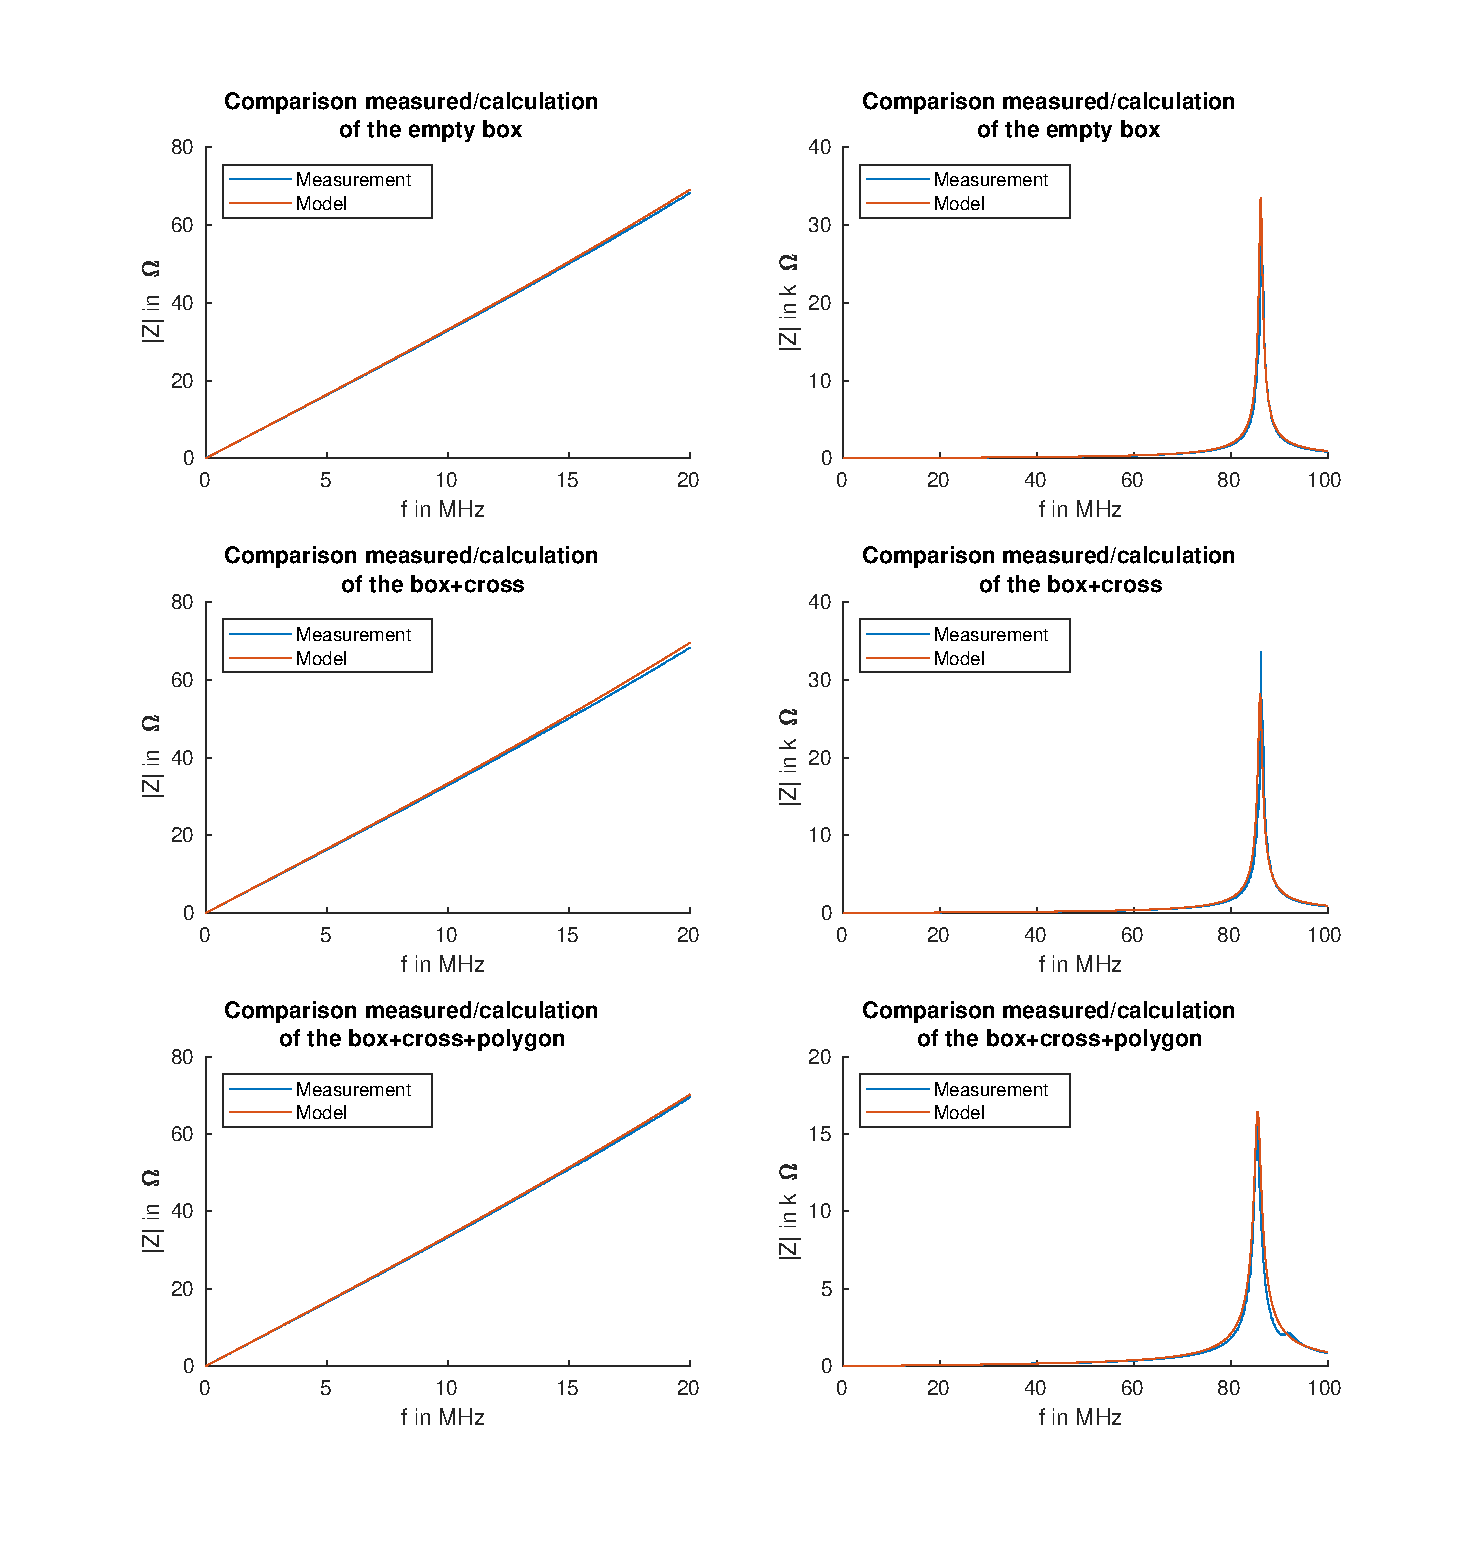
\includegraphics[width=\textwidth]{measurement_fit_ESB.eps}
	\caption{Gemessene Testboximpedanz mit gefitteter ESB-Impedanz}
	\label{fig:testboxfit}
\end{figure}
